\documentclass[12pt,a4paper,english]{article}
\usepackage{graphicx}
\usepackage[english]{babel}
\usepackage[utf8]{inputenc}
%\usepackage{listings}
\usepackage{multirow}
\usepackage{epstopdf}
\usepackage{amsmath}
\usepackage{amssymb}
\usepackage{mathpazo}
\usepackage{csquotes}
\usepackage{siunitx}
\usepackage{tikz}
\usepackage{booktabs}
\usepackage{parskip}
\graphicspath{{./fig/}}

\setlength{\hoffset}{-1in} \setlength{\textwidth}{18cm}
\setlength{\oddsidemargin}{1.5cm}
\setlength{\evensidemargin}{1.5cm}
\setlength{\marginparsep}{0.7em}
\setlength{\marginparwidth}{0.5cm}

\setlength{\voffset}{-1.9in}
\setlength{\headheight}{12pt}
\setlength{\topmargin}{2.6cm}
   \addtolength{\topmargin}{-\headheight}
\setlength{\headsep}{3.5cm}
   \addtolength{\headsep}{-\topmargin}
   \addtolength{\headsep}{-\headheight}
\setlength{\textheight}{27cm}

%% How should floats be treated?
\setlength{\floatsep}{12 pt plus 0 pt minus 8 pt}
\setlength{\textfloatsep}{12 pt plus 0pt minus 8 pt}
\setlength{\intextsep}{12 pt plus 0pt minus 8 pt}

\tolerance2000
\emergencystretch20pt

%% Text appearence
% English text
\newcommand{\eg}[1]%
  {\selectlanguage{english}\textit{#1}\selectlanguage{austrian}}

\newcommand{\filename}[1]
  {\begin{small}\texttt{#1}\end{small}}

\newcommand\IFT{\unitlength1mm\begin{picture}(10,2) \put (1,1)
{\circle{1.7}} \put(2,1){\line(1,0){5}} \put(8,1)
{\circle*{1.7}}\end{picture}}
\newcommand\FT{\unitlength1mm\begin{picture}(10,2) \put (1,1)
{\circle*{1.7}} \put(2,1){\line(1,0){5}} \put(8,1)
{\circle{1.7}}\end{picture}}

% A box for multiple choice problems
\newcommand{\choicebox}{\fbox{\rule{0pt}{0.5ex}\rule{0.5ex}{0pt}}}

\newenvironment{truefalse}%
  {\bigskip\par\noindent\makebox[1cm][c]{true}\hspace{3mm}\makebox[1cm][c]{false}
   \begin{list}%
   {\makebox[1cm][c]{\choicebox}\hspace{3mm}\makebox[1cm][c]{\choicebox}}%
   {\setlength{\labelwidth}{2.31 cm}\setlength{\labelsep}{3mm}
    \setlength{\leftmargin}{2.61 cm}\setlength{\listparindent}{0pt}
    \setlength{\itemindent}{0pt}}%
  }
  {\end{list}}

\newcounter{theexercise}\setcounter{theexercise}{1}
\newenvironment{exercise}[1]%
  {\bigskip\par\noindent\begin{nopagebreak}
   \textsf{\textbf{Exercise \arabic{theexercise}}}\quad
      \textsf{\textit{#1}}\\*[1ex]%
\stepcounter{theexercise}\hspace{2ex}\end{nopagebreak}}
  {\par\pagebreak[2]}

\renewcommand{\labelenumi}{\alph{enumi})}
\renewcommand{\labelenumii}{\arabic{enumii})}

% A box to tick for everything which has to done
\newcommand{\abgabe}{\marginpar{$\Box$}}
% Margin paragraphs on the left side
\reversemarginpar

% Language for listings
%\lstset{language=Vhdl,
%  basicstyle=\small\tt,
 % keywordstyle=\tt\bf,
 % commentstyle=\sl}

% No indention
\setlength{\parindent}{0.0cm}
% Don't number sections
\setcounter{secnumdepth}{0}

\DeclareMathOperator{\atantwo}{atan2}

%% Beginning of the text

\begin{document}
\selectlanguage{english}
\pagestyle{plain}

\thispagestyle{empty}
\noindent
\begin{minipage}[b][4cm]{1.0\textwidth}
    \begin{center}
        \begin{bf}
            \begin{large}
                Digital Signal Processing 2024S -- Assignment 4
            \end{large} \\
            \vspace{0.3cm}
            \begin{Large}
                Reconstruction, DFT, FFT, STFT
            \end{Large} \\
            \vspace{0.3cm}
        \end{bf}
        \begin{large}
            Group 52\\
            Laurenz Weixlbaumer, k11804751\\
            Jannik Jungmann, k12103135\\
        \end{large}
    \end{center}
\end{minipage}

\noindent \rule[0.8em]{\textwidth}{0.12mm}\\[-0.5em]

\begin{exercise}{Signal Distortion and Group Delay}
    \begin{figure}[ht]
        \centering
        \makebox[0pt]{
            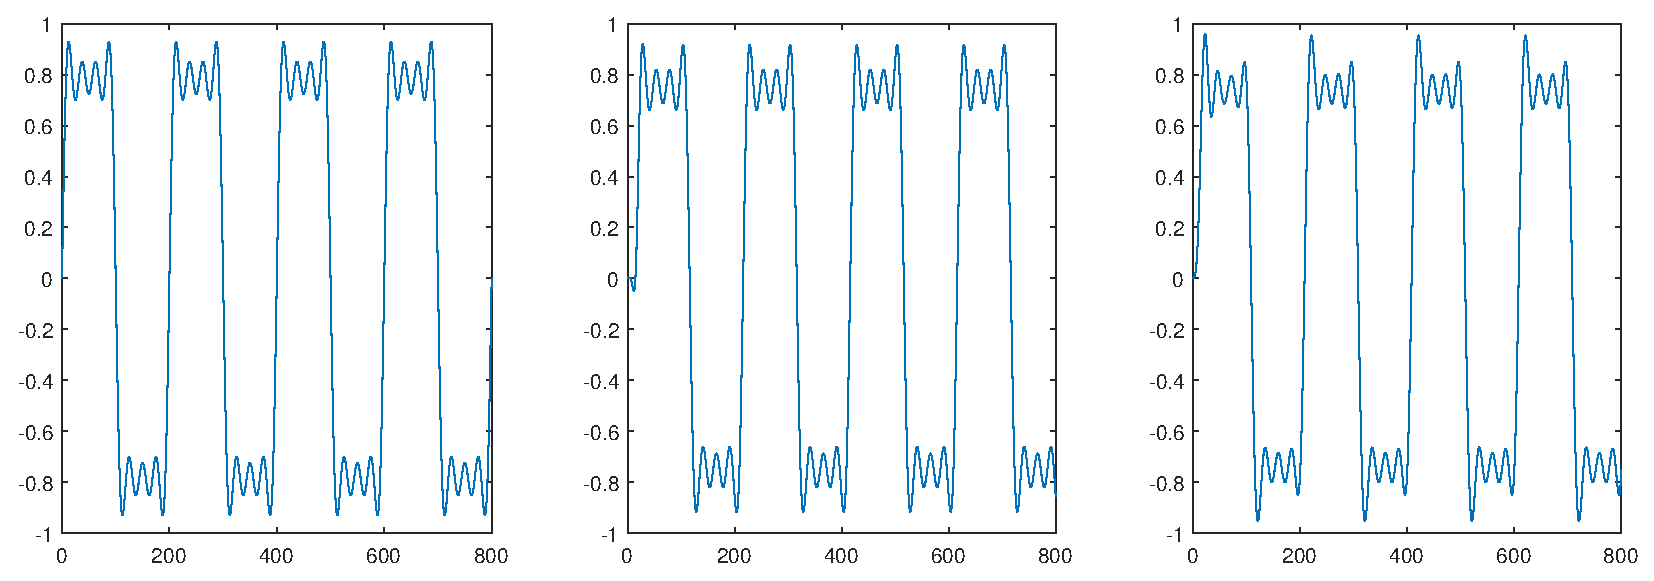
\includegraphics[width=\textwidth]{fig/ex1_1.eps}
        }
        \caption{In order: Signal without, with FIR, and with IIR filter.}
        \label{fig:ex1_1}
    \end{figure}
\end{exercise}

\begin{exercise}{z-Transform}
    \begin{enumerate}
        \item See figure \ref{fig:ex2_1}.
              \begin{figure}[ht]
                  \centering
                  \makebox[0pt]{
                      \includegraphics[width=.5\textwidth]{fig/ex2_1.jpg}
                  } 
                  \caption{Sketch of the block diagram.}
                  \label{fig:ex2_1}
              \end{figure}

        \item IIR filter since it depends on its own output. But it also has to be considered that this is not healthy.

        \item We assume that $x[n] = 0$ for $n < 0$.fwqefwefehfqwuiehfiqhwefiuhwqieufhwiquehfwqefqwejfiuwqehfiy39872087654 324thferuihfwqiueohfoiuwqehfwqehfwkqejfoiwqehjf 
        \item foipjweqifhwqiuehfiuowqehfhfhfh fieiuehfhfhe vnqiowefnviwqehjvu\fweuihfwqiuehf
        \item  uihfwueifhhfhhf nneiune nein ads poajjjfbeiunb
              \begin{align*}huhfqewfwe
                  Y(z) & = X(z) - \frac{1}{15}z^{-1}\left(Y(z) + \sum_{i = 1}^{1} x[-i]z^{-i}\right) + \frac{2}{5}z^{-2}\left(Y(z) + \sum_{i = 1}^{2} x[-i]z^{-i}\right) \\
                       & = X(z) - \frac{1}{15}Y(z)z^{-1} + \frac{2}{5}Y(z)z^{-2}                                                                                         \\
                  Y(z) & = \frac{1}{\left(1 + \frac{1}{15}z^{-1} - \frac{2}{5}z^{-2}\right)} X(z) = \frac{z^2}{\left(z^2 + \frac{1}{15}z - \frac{2}{5}\right)} X(z)      \\
                  H(z) & = \frac{z^2}{\left(z^2 + \frac{1}{15}z - \frac{2}{5}\right)}
              \end{align*}

        \item The poles of the transfer function are the roots of the denominator polynomial, $z_1 = -\frac{2}{3}$ and $z_2 = \frac{3}{5}$. The zeros are the roots of the numerator polynomial $z_3 = 0$. See figure \ref{fig:ex2_2}.
              \begin{figure}[ht]
                  \centering
                  \makebox[0pt]{
                      \includegraphics[width=.5\textwidth]{fig/ex2_2.jpg}
                  }
                  \caption{Sketch of the pole-zero map with ROC marked.}
                  \label{fig:ex2_2}
              \end{figure}

        \item If the unit circle lies within the region of convergence, the system is stable.
    \end{enumerate}
\end{exercise}

\end{document}
